\section{含参问题}
\label{sec:sens-problems}

参数变化之后，“解的变化”到底指什么？本节要先回答这个问题。参数一变，问题可能没有解，也可能有许多解，所以必须先把比较的对象定义清楚。

\paragraph{贯穿全章的预算二次例}
沿用第~\ref{chap:constrained-optimality}章的预算分配。两种投入的数量是$x_1$、$x_2$，它们非负，总量不超过预算$\tau$。理想配置是$(2,1)$，偏离理想配置按平方计算损失。于是得到问题
\begin{equation}
 \min_{\bm{x}\in\mathbb{R}^2}\ \frac12(x_1-2)^2+\frac12(x_2-1)^2
 \quad\text{s.t.}\quad x_1+x_2\leq\tau,\ \ x_1\geq0,\ \ x_2\geq0.
 \label{eq:sens-budget}
\end{equation}
为了和一般记号对应，把三条约束写成$g_1=x_1+x_2-\tau$、$g_2=-x_1$、$g_3=-x_2$，都要求不大于零，相应的乘子是$\lambda_1,\lambda_2,\lambda_3$。

这个问题有清楚的几何图景。目标的等高线是以理想点$\bm{c}=(2,1)$为圆心的同心圆，所以最优解就是可行三角形里离$\bm{c}$最近的点。预算线像一堵可以平移的墙，$\tau$增大时墙向外退，三角形变大。

图~\ref{fig:sens-budget-family}画出三个预算水平。$\tau=4$时墙退得很远，碗底$(2,1)$本身可行，没有约束起作用。$\tau=2$时碗底被挡在墙外，解落在预算线上的$(3/2,1/2)$。$\tau=0.5$时三角形很小，解被挤到角点$(0.5,0)$，预算和$x_2\geq0$同时起作用。

\begin{BookInlineFigure}
 \centering
 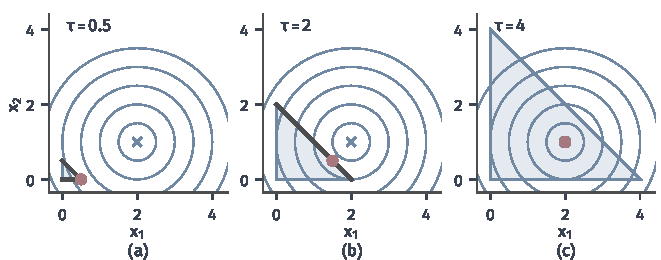
\includegraphics[width=112mm]{figures/05-optimization/06-constrained-optimization/matplotlib/sens-budget-family/figure.pdf}
 \caption{预算二次例~\eqref{eq:sens-budget}在三个预算下的情形。浅蓝三角形是可行集，蓝色同心圆是目标等高线，蓝色叉是理想点$(2,1)$，红点是最优解，深灰粗线是起作用的约束。(a)~$\tau=0.5$，预算和$x_2\geq0$都起作用。(b)~$\tau=2$，只有预算起作用。(c)~$\tau=4$，没有约束起作用。}
 \label{fig:sens-budget-family}
\end{BookInlineFigure}

\paragraph{变量与参数}
式~\eqref{eq:sens-budget}里有两类量。$\bm{x}$由优化决定，$\tau$由外部给定，求解时保持不变。前者是我们的选择，后者是我们所处的环境。同一个量算变量还是参数，取决于建模时想回答什么：若预算也可以选择，它就应该成为变量。

把环境写成参数向量$\bm{\theta}$，每个$\bm{\theta}$确定一个优化问题，全体构成一族问题。研究这族问题，需要两个输出对象。

\begin{definition}[含参问题、最优值函数与解映射]
\label{def:sens-family}
设$\bm{\Theta}\subseteq\mathbb{R}^q$是参数集合。对每个$\bm{\theta}\in\bm{\Theta}$，给定可行集$\bm{C}(\bm{\theta})\subseteq\mathbb{R}^n$和目标$f(\cdot,\bm{\theta})$，称
\begin{equation}
 \min_{\bm{x}\in\bm{C}(\bm{\theta})}f(\bm{x},\bm{\theta})
 \label{eq:sens-family}
\end{equation}
为\term{含参问题}（parametric problem）。函数
\begin{equation}
 V(\bm{\theta})=\inf_{\bm{x}\in\bm{C}(\bm{\theta})}f(\bm{x},\bm{\theta})
 \label{eq:sens-value}
\end{equation}
称为\term{最优值函数}（value function），并约定空集上的下确界为$+\infty$。把每个参数对应到最优解集合的映射
\begin{equation}
 \bm{S}(\bm{\theta})=\bigl\{\bm{x}\in\bm{C}(\bm{\theta}):f(\bm{x},\bm{\theta})=V(\bm{\theta})\bigr\}
 \label{eq:sens-solution-map}
\end{equation}
称为\term{解映射}（solution map）。
\end{definition}

$V$和$\bm{S}$的性格很不一样。$V(\bm{\theta})$总是一个确定的量，只是可能取$\pm\infty$。$\bm{S}(\bm{\theta})$是一个集合，可能是空集，可能只有一个点，也可能有无穷多个点。对预算例，$\tau<0$时可行集是空集，所以$V(\tau)=+\infty$，$\bm{S}(\tau)=\varnothing$。$\tau\geq0$时目标强凸、可行集紧，$\bm{S}(\tau)$恰有一个点。

\paragraph{参数改变可能使问题失去解}
除了不可行，参数改变还可能让最小值取不到。下面的一族问题定义在整条实轴上：
\[
 \min_{x\in\mathbb{R}}\ f(x,\theta)=e^{x}-\theta x.
\]
图~\ref{fig:sens-three-outcomes}画出三种情况，下面逐个计算。

\begin{BookInlineFigure}
 \centering
 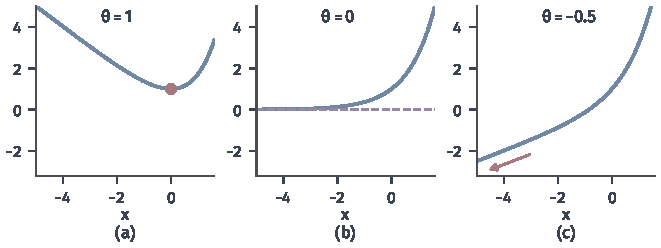
\includegraphics[width=112mm]{figures/05-optimization/06-constrained-optimization/matplotlib/sens-three-outcomes/figure.pdf}
 \caption{同一族目标$f(x,\theta)=e^{x}-\theta x$在三个参数下的结果。(a)~$\theta=1$，最小值$1$在红点$x=0$取得。(b)~$\theta=0$，下确界$0$（紫色虚线）有限但取不到。(c)~$\theta=-0.5$，红色箭头表示目标沿$x\to-\infty$无下界。}
 \label{fig:sens-three-outcomes}
\end{BookInlineFigure}

$\theta>0$时，令导数$e^x-\theta$为零，得到唯一的驻点$x=\ln\theta$。二阶导数$e^x$为正，所以它是全局极小点，并且
\[
 V(\theta)=\theta-\theta\ln\theta,\qquad \bm{S}(\theta)=\{\ln\theta\}.
\]

$\theta=0$时目标是$e^x$，它的下确界是$0$，但没有点取得这个值，所以$V(0)=0$而$\bm{S}(0)=\varnothing$。$\theta<0$时，$x\to-\infty$使$-\theta x=\lvert\theta\rvert x\to-\infty$，而$e^x\to0$，所以$V(\theta)=-\infty$。

这族问题还显示出值与解的差别。$\theta\downarrow0$时，$V(\theta)=\theta-\theta\ln\theta\to0=V(0)$，值的变化是连续的。解却是$\ln\theta\to-\infty$，一路跑向无穷远。讨论变化之前，必须先确认所研究的$\bm{\theta}$处解存在，并说明比较的是值还是解。

\paragraph{有多个解时要说清跟踪谁}
考虑一个有两个山谷的目标：
\begin{equation}
 f(x,\theta)=(x^2-1)^2+\theta x.
 \label{eq:sens-double-well}
\end{equation}
$\theta=0$时两个谷底$x=\pm1$同样低，$\bm{S}(0)=\{-1,1\}$。$\theta$不为零时，$\theta x$这一项把地面倾斜，一个谷底升高，另一个降低。“最优解对$\theta$的导数”这句话在$\theta=0$处没有明确含义，因为不知道说的是哪一个解。

这时有两种办法把问题说清楚。一种是跟踪一条\term{局部极小分支}（local minimizer branch），即在$\bm{\theta}_0$的邻域上定义的映射$\bm{x}(\bm{\theta})$，使每个$\bm{x}(\bm{\theta})$都是相应问题的局部极小点，并且随$\bm{\theta}$连续变化。另一种是约定\term{选解规则}（selection rule），例如总取最优解中范数最小的一个。

沿分支的目标值记作
\begin{equation}
 v(\bm{\theta})=f(\bm{x}(\bm{\theta}),\bm{\theta}).
 \label{eq:sens-branch-value}
\end{equation}
小写的$v$是某条分支上的值，大写的$V$是全局最优值。分支上的点都可行，所以$v(\bm{\theta})\geq V(\bm{\theta})$，只有分支恰好全局最优时才取等号。

图~\ref{fig:sens-double-well}展示了这种区别。(b)中两条绿色虚线是两个谷底的位置，它们各自光滑。红色实线是全局最优解，它在$\theta=0$处从上面一条跳到下面一条。(c)中分支的值光滑地穿过$\theta=0$，全局最优值是两者中较小的那个，在$\theta=0$处有折角。例如沿右侧谷底的分支在$\theta>0$时仍然是局部极小，但它的值已经高于全局最优值，不能称为“最优值”。

\begin{BookInlineFigure}
 \centering
 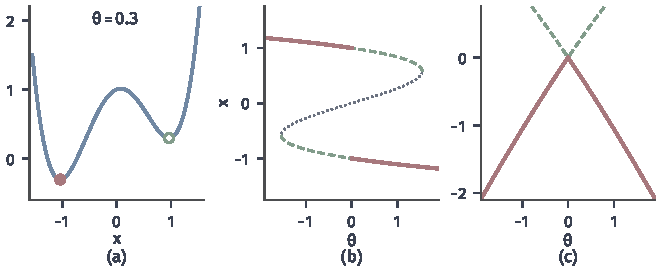
\includegraphics[width=112mm]{figures/05-optimization/06-constrained-optimization/matplotlib/sens-double-well/figure.pdf}
 \caption{双谷目标~\eqref{eq:sens-double-well}的分支与全局解。(a)~$\theta=0.3$时的目标，红点是全局最小点，绿色空心点是另一个局部极小点。(b)~驻点随$\theta$的变化：绿色虚线是局部极小分支，灰色点线是局部极大分支，红色实线是全局最优解。(c)~绿色虚线是两条分支上的目标值，红色实线是全局最优值。}
 \label{fig:sens-double-well}
\end{BookInlineFigure}

图~\ref{fig:sens-objects}汇总这些对象的关系。本章每个结论都会说明针对哪一个对象：是全局的$V$，还是某条分支上的$v$；是整个解集合$\bm{S}$，还是分支$\bm{x}(\bm{\theta})$。

\begin{BookInlineFigure}
 \centering
 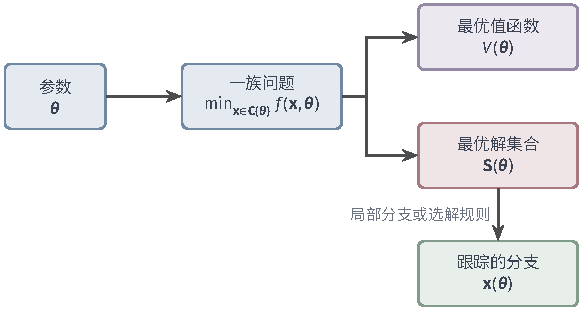
\includegraphics[width=99mm]{figures/05-optimization/06-constrained-optimization/tikz/sens-objects/figure.pdf}
 \caption{含参问题的三个输出对象。参数确定一个优化问题，问题确定最优值函数和最优解集合。解集合可能为空或含多个点，只有通过局部分支或选解规则，才得到一个随参数变化的点。}
 \label{fig:sens-objects}
\end{BookInlineFigure}
